% Replication of Favara and Imbs (2015): Problem Set 3, Empirical Methods (UZH, HS 2026)
% Compile with pdfLaTeX. Needs tables/ and figures/ next to this file.
\documentclass[12pt,a4paper]{article}

\usepackage[utf8]{inputenc}
\usepackage[T1]{fontenc}
\usepackage{mathptmx}
\usepackage{microtype}
\usepackage[margin=2.5cm]{geometry}
\usepackage{amsmath,amssymb}
\usepackage{graphicx}
\usepackage{booktabs}
\usepackage{tabularx}
\usepackage{array}
\usepackage{colortbl}
\usepackage{enumitem}
\usepackage{xcolor}
\usepackage[font=small,labelfont=bf,skip=6pt]{caption}
\usepackage[hidelinks]{hyperref}

\setlength{\parindent}{0pt}
\setlength{\parskip}{6pt}

% --- Helpers for the worksheets --------------------------------------------
\newcolumntype{L}{>{\raggedright\arraybackslash}X}
\newcolumntype{P}[1]{>{\raggedright\arraybackslash}p{#1}}
\newcommand{\fillrow}{\rule[-0.35cm]{0pt}{0.85cm}}  % leaves room to write in a row
\newcommand{\rowline}{\arrayrulecolor{black!25}\hline\arrayrulecolor{black}}
\renewcommand{\arraystretch}{1.25}

% --- Table notes -----------------------------------------------------------
\newcommand{\tablenotes}[1]{\par\vspace{4pt}{\footnotesize\textit{Notes:} #1\par}}

\graphicspath{{figures/}}
\renewcommand{\topfraction}{0.9}
\renewcommand{\bottomfraction}{0.8}
\renewcommand{\textfraction}{0.07}
\renewcommand{\floatpagefraction}{0.85}
\title{Replication of Favara and Imbs (2015):\\{} Credit Supply and the Price of Housing}
\author{%
  Riccardo Balestra (23732522), Raphael Frei (21612379),\\
  Levin Gashi (23723802), Pascal Dietz (21608757)\\[0.4em]
  \small Replication package: \url{https://github.com/Duki-cybar/favara-imbs-replication}.\\
  \small Run \texttt{run\_all.py} to reproduce all tables and figures; see the README for details.%
}
\date{}

\begin{document}
\maketitle

\begin{abstract}
Favara and Imbs (2015) use the removal of interstate branching restrictions in US states between 1994 and 2005 as an instrument for mortgage credit and conclude that more credit supply leads to higher house prices. With the authors' replication package we reproduce their main IV estimate of 0.141 exactly. We then show that this estimate is fragile. It is no longer significant when we cluster standard errors by state, it turns negative if the state weights are dropped, and with public FHFA house price data the point estimate falls to 0.05 and is insignificant.
\end{abstract}

% ===========================================================================
\section{Introduction}
% ===========================================================================

Mortgage credit and house prices both grew strongly in the US before 2006. The problem in testing whether credit pushed up prices is that the causality could also go the other way: when house prices rise, people need bigger loans and banks are happy to lend against more valuable collateral. Favara and Imbs (2015) try to solve this with a policy change. The Interstate Banking and Branching Efficiency Act (IBBEA) of 1994 allowed banks to open branches in other states, but each state could keep up to four restrictions against out-of-state banks. States dropped these restrictions in different years, and only commercial banks were affected. Independent mortgage companies, thrifts and credit unions were not. The authors show that commercial banks lend more after deregulation while the other lenders do not, and then use the deregulation index as an instrument for credit growth in a panel of US counties (1994--2005). They find an elasticity of house prices to credit of about 0.14, which is larger in counties where it is hard to build new houses.

We replicate the first stage (their Table~2), the main IV table (Table~5) and the impulse responses (Figure~3). Since the instrument only changes at the state level, most of our evaluation is about the standard errors and about whether deregulation could affect house prices through other channels than mortgage credit. For our extension we replace the house price data from Moody's, which are not publicly available, with the public county index of the Federal Housing Finance Agency (FHFA).

% ===========================================================================
\section{Data and Methodology}
% ===========================================================================

\subsection{Data}

All data come from the authors' replication package on openICPSR, which already contains a county-year panel. Mortgage lending is taken from the HMDA records. The authors measure it in three ways: the number of new loans, the loan volume and the loan-to-income ratio, each in log changes and separately for commercial banks and for the placebo lenders. The house price series from Moody's Economy.com is the median price of existing single-family homes and is available for roughly 1,000 urban counties. The instrument is the index of Rice and Strahan (2010), which counts the four restrictions a state kept (minimum age of the target bank, ban on de novo branching, ban on buying single branches, deposit cap). The authors use four minus this index, so 0 means fully restricted and 4 means fully open. As controls they use the growth of income per capita and population and the change in a Herfindahl index of mortgage originations, each current and lagged. Supply elasticities are from Saiz (2010).

The package already contains the lagged variables, the instrument and the state weights, so our own data work consists of merging the three county-year files as in the authors' \texttt{master.do}. Our final IV sample has 11,107 county-years and 1,018 counties, the same as in the paper. For the extension we downloaded the FHFA annual county index, computed its log changes and their lag ourselves, and merged it on county FIPS code and year.

\subsection{Empirical strategy}

The model is estimated by 2SLS with county and year fixed effects. For county $c$ in state $s$ in year $t$ the two stages are
\begin{align}
  \Delta \log L_{ct} &= \alpha_c + \lambda_t + \pi\, D_{s,t-1} + \rho_1 \Delta \log P_{c,t-1} + \gamma_1' W_{ct} + u_{ct}, \label{eq:fs}\\
  \Delta \log P_{ct} &= \alpha_c + \lambda_t + \beta\, \widehat{\Delta \log L}_{ct} + \rho_2 \Delta \log P_{c,t-1} + \gamma_2' W_{ct} + \varepsilon_{ct}, \label{eq:main}
\end{align}
where $L_{ct}$ is mortgage credit by commercial banks, $P_{ct}$ the house price index, $D_{s,t-1}$ the deregulation index of the previous year and $W_{ct}$ the controls. The county effects take out anything that is constant in a county, like its geography, and the year effects take out shocks that hit all counties at once, for example changes in interest rates. What is left to identify $\beta$ is the part of credit growth that follows a state's own deregulation, so in the end counties in states that already deregulated are compared to counties in states that had not yet done so. The regressions are weighted with the inverse of the number of counties in the state. The authors do this because otherwise states with many counties would dominate the estimate, and in their view these are exactly the states where the response of house prices is most heterogeneous.

For $\beta$ to be causal the instrument has to be relevant and exogenous. Relevance means that deregulation actually changes credit growth, which can be tested (Table~\ref{tab:placebo}). Exogeneity is harder. States must not have chosen the timing of deregulation because of what was going on in their housing markets, and deregulation must affect house prices only through mortgage credit. The authors' main argument is the placebo test: if deregulation just coincided with high housing demand, all lenders should lend more, not only commercial banks. Prices also react less where housing supply is elastic, as expected if credit raises housing demand.

% ===========================================================================
\section{Main Result}
% ===========================================================================

\subsection{Replication}

Table~\ref{tab:main} shows our version of Table~5. The coefficients are 0.141, 0.135 and 0.120, compared with 0.141, 0.134 and 0.120 in the paper, and the standard errors differ by at most 0.001. The first-stage $F$-statistics are slightly higher in our case (for example 10.15 instead of 10.13), which we attribute to small differences in degrees-of-freedom corrections between Stata and our own Python estimator (written with \texttt{numpy}, since we found no package that reproduces the panel HAC errors of \texttt{xtivreg2} exactly). To get this close, two settings from the authors' Stata code are needed: the state weights and HAC standard errors within each county (Bartlett kernel with bandwidth 3, as in \texttt{xtivreg2} with \texttt{bw(3)}). Table~\ref{tab:robust} shows how much the results change without them. With these settings, Table~\ref{tab:placebo} matches the paper exactly and the reduced-form coefficients differ by at most 0.0001.

\begin{table}[!htbp]
  \centering
  \caption{House prices and instrumented credit growth (replication of Table 5)}
  \label{tab:main}
  \begin{tabular}{lccc}
\toprule
 & (1) & (2) & (3) \\
 & Number of loans & Loan volume & Loan to income \\
\midrule
Instrumented credit growth & 0.141** & 0.135** & 0.120** \\
 & (0.069) & (0.063) & (0.058) \\
Lagged house price & 0.507*** & 0.456*** & 0.472*** \\
 & (0.029) & (0.040) & (0.038) \\
\midrule
Paper: credit growth & 0.141 & 0.134 & 0.120 \\
 & (0.069) & (0.062) & (0.057) \\
\midrule
First-stage $F$ & 10.15 & 10.33 & 8.61 \\
First-stage $F$ (paper) & 10.13 & 10.31 & 8.59 \\
Observations & 11,107 & 11,107 & 11,107 \\
Counties & 1,018 & 1,018 & 1,018 \\
\bottomrule
\end{tabular}
  \tablenotes{Second stage of 2SLS regressions of the log change in the county house price
  index on the log change in mortgage credit of commercial banks: number of loans (1), loan
  volume (2), loan-to-income ratio (3). Credit growth is instrumented with the lagged
  interstate branching deregulation index (Rice and Strahan, 2010). All regressions include
  county fixed effects, year dummies, the lagged house price change and income, population
  and Herfindahl controls, and are weighted by the inverse number of counties per state.
  Sample: US urban counties, 1994--2005. HAC standard errors (Bartlett kernel, bandwidth 3)
  in parentheses. *** $p<0.01$, ** $p<0.05$, * $p<0.1$.}
\end{table}

Figure~\ref{fig:main} is our replication of Figure~3, estimated with local projections (Jord\`a, 2005). The effect of credit on house prices is 0.14 in the first year, gets bigger until about 0.26 after two years and then becomes smaller again. After seven years it is slightly negative. This fits with our replication of the paper's Figure~1 (in our repository), where credit growth goes up by about three percent after a deregulation step but the effect is gone after around four years. Given Section~\ref{sec:threats}, these robust-SE bands (as used by the authors) are likely too narrow.

\begin{figure}[!htbp]
  \centering
  \caption{House prices: impulse responses to an instrumented credit shock (replication of Figure 3)}
  \label{fig:main}
  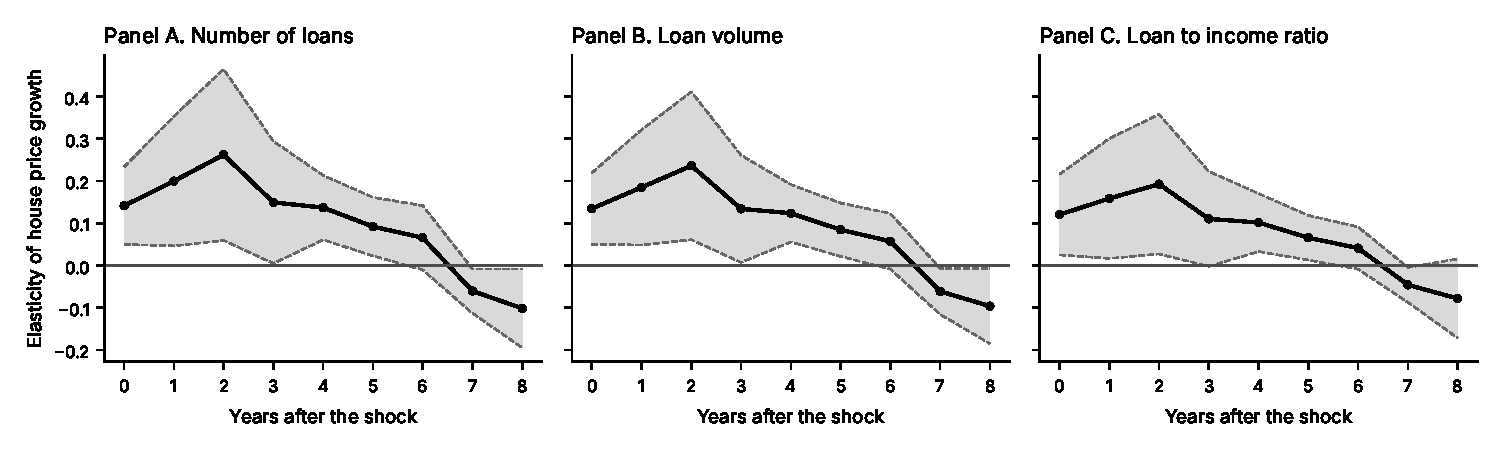
\includegraphics[width=\textwidth]{figure3_irf_house_prices.pdf}
  \tablenotes{Local projections (Jord\`a, 2005): coefficient on instrumented credit growth in
  2SLS regressions of the house price change $h = 0,\dots,8$ years ahead, same specification as
  Table~\ref{tab:main} but with heteroskedasticity-robust standard errors (no autocorrelation or
  state clustering), as in the authors' code. Shaded areas: 90 percent confidence bands.}
\end{figure}

\subsection{Interpretation}

Because both sides are in log changes, $\beta$ can be read as an elasticity. When the number of mortgage loans grows by one percentage point more, house prices grow by about 0.14 percentage points more in the same year, holding the other variables constant. The lagged house price has a coefficient of 0.51, so price growth is quite persistent, and a lasting increase in credit growth would have a long-run effect of around $0.141/(1-0.507)\approx 0.29$. In the reduced form (paper's Table~4, column~1), one more restriction removed goes along with about one percentage point higher house price growth per year (coefficient 0.0103).

The OLS estimate on the same sample is only 0.005, about 30 times smaller. Weak-instrument bias goes towards OLS and cannot explain this. More likely are measurement error in the HMDA data (attenuating OLS), a local average treatment effect for counties whose credit reacts to deregulation, or a violated exclusion restriction (below).

% ===========================================================================
\section{Critical Evaluation}
% ===========================================================================

\subsection{Threats to internal validity}
\label{sec:threats}

\textit{Standard errors.} In our view this is the biggest problem. The deregulation index is the same for all counties of a state, but the HAC standard errors only allow the errors of one county to be correlated over time. Counties in the same state get the same policy shock and probably also share other shocks, for example in the state labor market, so their errors are likely correlated as well. Bertrand et al.\ (2004) show that ignoring this can make standard errors much too small. When we cluster by state (Table~\ref{tab:robust}), the coefficient stays at 0.141 but the standard error goes from 0.069 to 0.129 and the result is not significant anymore. The first-stage $F$ also drops from 10.2 to 4.3, which is well below the rule-of-thumb value of 10 (Stock et al., 2002). Because of this we also computed Anderson--Rubin (1949) confidence sets, which are valid with weak instruments. With HAC errors they do not include zero, but with state clusters they do for all three credit measures, and for the number of loans the set has no upper bound. The first stage in Table~\ref{tab:placebo} is already clustered by state and not affected.

\begin{table}[!htbp]
  \centering
  \caption{Commercial banks versus placebo lenders (replication of Table 2)}
  \label{tab:placebo}
  \begin{tabular}{lccc}
\toprule
 & Number of loans & Loan volume & Loan to income \\
\midrule
Commercial banks: deregulation & 0.028** & 0.029** & 0.029** \\
 & (0.010) & (0.012) & (0.011) \\
\quad paper & 0.028 (0.010) & 0.029 (0.012) & 0.029 (0.011) \\
\quad observations & 10,992 & 10,992 & 10,991 \\
Placebo lenders: deregulation & 0.002 & 0.001 & 0.001 \\
 & (0.008) & (0.008) & (0.008) \\
\quad paper & 0.002 (0.008) & 0.001 (0.008) & 0.001 (0.008) \\
\quad observations & 10,580 & 10,580 & 10,579 \\
\bottomrule
\end{tabular}
  \tablenotes{Fixed-effects regressions of the log change in mortgage lending on the lagged
  deregulation index, a lagged dependent variable, and income, population, house price and
  Herfindahl controls (current and lagged), with county and year fixed effects, unweighted as
  in the original. Placebo lenders: independent mortgage companies, thrifts and credit unions.
  Standard errors clustered by state in parentheses. ** $p<0.05$, *** $p<0.01$.}
\end{table}

\textit{Simultaneity.} Credit and prices are determined jointly, which is why the authors use IV. This only works if states did not deregulate because their housing markets were booming. Our anticipation test (in our repository) supports them: future deregulation steps predict neither credit growth nor house price growth.

\textit{Exclusion restriction.} The placebo test shows that deregulation changed credit supply. It does not show that credit supply was the only way deregulation affected house prices. Rice and Strahan (2010) find that interstate branching also made credit cheaper for small firms. If local firms grow and pay higher wages because of this, demand for housing rises even without any change in mortgage lending. Let $\delta$ be this direct effect of $D$ on house price growth, which ends up in $\varepsilon$. Then
\begin{equation}
  \operatorname{plim} \hat\beta_{IV} = \beta + \frac{\operatorname{Cov}(\tilde D, \varepsilon)}{\operatorname{Cov}(\tilde D, \Delta \log \tilde L)} = \beta + \frac{\delta}{\pi}, \label{eq:bias}
\end{equation}
where the tildes denote residuals after the fixed effects and controls and $\pi$ is the first-stage coefficient. With $\delta>0$ and $\pi>0$ the bias is upward. Because $\hat\beta_{IV}$ is the reduced form $\rho$ divided by $\pi$, the bias as a share of the estimate is simply $\delta/\rho$. The reduced-form effect is about one percentage point per year. If only 0.3 points of it came through higher incomes rather than mortgages, the true elasticity would be about 0.10 instead of 0.14, and with 0.5 points it would be halved. The authors control for income growth, but income could itself be affected by deregulation (a ``bad control''), so it is not clear that this control solves the problem.

\textit{Choices in the specification.} Some other results in Table~\ref{tab:robust} are worth pointing out. Without the state weights the coefficient is $-0.034$ and significant, so the positive effect only appears when small states with few counties get as much weight as large ones. This is not a weak-instrument problem, since the unweighted first stage is much stronger ($F = 43$). It rather suggests that the effect is very heterogeneous and that 0.14 is an average dominated by states with few counties. If the lagged house price is dropped, the estimate more than doubles. A lagged dependent variable with county fixed effects in a short panel ($T \le 12$) causes Nickell (1981) bias of order $1/T$, downward in the persistence coefficient and spilling over to $\beta$; the authors' addendum (Favara and Imbs, 2015, Addendum) addresses this with GMM. Splitting at the median Saiz elasticity gives 0.070 (inelastic) and $-0.031$ (elastic): the expected ranking, but both insignificant with weak first stages. The reduced-form interaction ($-0.0084$) supports the mechanism more clearly.

\begin{table}[!htbp]
  \centering
  \caption{Robustness of the IV estimate (Table 5, column 1)}
  \label{tab:robust}
  \small
  \begin{tabular}{lccc}
\toprule
\multicolumn{4}{l}{\textit{2SLS, number of loans}} \\
Specification & Coefficient (SE) & First-stage $F$ & Obs. \\
\midrule
Baseline (Table 5, col. 1) & 0.141** (0.069) & 10.2 & 11,107 \\
Without lagged house price & 0.315** (0.126) & 11.1 & 11,107 \\
Only lagged house price as control & 0.125** (0.053) & 16.9 & 11,110 \\
No controls & 0.303*** (0.081) & 23.9 & 12,013 \\
OLS (no instrument) & 0.005*** (0.001) & -- & 11,107 \\
Unweighted (no $w_1$) & -0.034** (0.014) & 43.1 & 11,107 \\
SEs clustered by state & 0.141 (0.129) & 4.3 & 11,107 \\
Inelastic supply (below median) & 0.070 (0.058) & 7.9 & 4,851 \\
Elastic supply (above median) & -0.031 (0.045) & 4.3 & 4,829 \\
\midrule
\multicolumn{4}{l}{\textit{95\% confidence sets}} \\
Credit measure & Wald (HAC) & AR (HAC) & AR (state clusters) \\
\midrule
Number of loans & [0.01, 0.28] & [0.05, 0.44] & [-0.03, 3.00]$^{a}$ \\
Loan volume & [0.01, 0.26] & [0.05, 0.40] & [-0.03, 1.81] \\
Loan to income & [0.01, 0.23] & [0.04, 0.40] & [-0.03, 1.03] \\
\bottomrule
\end{tabular}
  \tablenotes{Each row changes one element of the baseline 2SLS specification of
  Table~\ref{tab:main}, column 1 (number of loans). Unless stated otherwise, standard errors
  are HAC within county (Bartlett kernel, bandwidth 3). Dropping controls changes the sample
  (rows 3 and 4) because fewer observations have missing values. The elasticity split uses
  only counties with a Saiz elasticity. AR: Anderson--Rubin confidence set, robust to weak
  instruments. $^{a}$ The set reaches the upper end of the search grid (3.0), i.e.\ it is
  unbounded above. * $p<0.1$, ** $p<0.05$, *** $p<0.01$.}
\end{table}

\subsection{Overall assessment}

The first part of the paper is convincing: deregulation raised lending by commercial banks but not by other lenders, also with clustered errors. The house price effect is not significant once errors are clustered at the level of the instrument and depends on the weights, so we read 0.14 as an indication that credit matters rather than a precise number.

% ===========================================================================
\section{Extension and Robustness}
% ===========================================================================

\subsection{Extension}

All results in the paper use Moody's house prices, which we could only use through the replication package. We wanted to know if the result also holds with data anyone can download, so we estimated equation~\eqref{eq:main} again with the FHFA county index. It is a repeat-sales index, so it compares the same house at two sales and is not affected by which houses are sold in a year; it only covers Fannie Mae and Freddie Mac mortgages and includes refinancing appraisals. Nothing else in the specification changes. Because FHFA does not cover all counties in every year, we also ran the Moody's regression on exactly the same 10,272 county-years. If both indices measured the same prices with some random noise, the two coefficients should be close, since noise in the dependent variable does not bias $\beta$.

With FHFA prices the coefficient for the number of loans is 0.054 and not significant, while Moody's gives 0.169 on the same observations (Table~\ref{tab:ext}). The same pattern holds for the other two credit measures. One explanation could be that more credit changes which houses are sold. If buyers can borrow more and buy bigger or more expensive houses, the median price goes up even when the price of a given house does not change much. The FHFA index would not show this. Its limited coverage and the refinancing appraisals could also play a role. The authors write that their results hold with the CoreLogic index, which also holds quality constant, but we could not check this because the data are not public.

\begin{table}[!htbp]
  \centering
  \caption{Extension: public FHFA house prices instead of Moody's}
  \label{tab:ext}
  \begin{tabular}{lccc}
\toprule
 & Number of loans & Loan volume & Loan to income \\
\midrule
FHFA house prices & 0.054 & 0.050 & 0.045 \\
 & (0.058) & (0.052) & (0.045) \\
\quad first-stage $F$ / obs. & 5.5 / 10,272 & 5.9 / 10,272 & 4.9 / 10,272 \\
Moody's, FHFA sample & 0.169* & 0.155* & 0.136* \\
 & (0.092) & (0.080) & (0.072) \\
\quad first-stage $F$ / obs. & 7.2 / 10,272 & 7.8 / 10,272 & 6.4 / 10,272 \\
\bottomrule
\end{tabular}
  \tablenotes{2SLS as in Table~\ref{tab:main}. First row: outcome is the log change in the FHFA
  annual county house price index (all transactions, developmental). Second row: Moody's
  index on exactly the same county-years. HAC standard errors (Bartlett kernel, bandwidth 3)
  in parentheses. * $p<0.1$, ** $p<0.05$, *** $p<0.01$.}
\end{table}

The strength of the extension is that it uses public data and holds the sample fixed. Its limits are weak first stages ($F$ of 5--8) and that we have not tested the difference formally: treating the two estimates as independent, the gap of 0.115 has a standard error of about 0.11. Since they are positively correlated the true one is smaller, so a stacked regression would be the next step.

\subsection{Ideal empirical strategy}

Ideally, we would run an experiment. A regulator would make mortgages easier to get, for example by allowing a higher loan-to-value ratio, in a random half of several hundred similar local housing markets and keep the old rules in the other half. With random assignment the timing could not depend on local conditions, and since nothing else changes, the exclusion restriction would hold by design. We would measure the outcome with actual sale prices, so the choice of index would not matter, and cluster the standard errors by housing market.

% ===========================================================================
\section{Conclusion}
% ===========================================================================

We replicate the main results of Favara and Imbs (2015) almost exactly. The evidence that branching deregulation increased credit supply by commercial banks is strong. The effect on house prices is less robust: it is not significant with standard errors clustered by state, it depends on the state weights, and with FHFA house prices it is only about one third as large. Credit supply probably did raise house prices, but the size of the effect is less certain than the paper's main table suggests.

% ===========================================================================
\begin{thebibliography}{0}
% ===========================================================================
\bibitem{anderson1949} Anderson, T. W., \& Rubin, H. (1949). Estimation of the parameters of a single equation in a complete system of stochastic equations. \textit{Annals of Mathematical Statistics}, 20(1), 46--63.
\bibitem{bertrand2004} Bertrand, M., Duflo, E., \& Mullainathan, S. (2004). How much should we trust differences-in-differences estimates? \textit{Quarterly Journal of Economics}, 119(1), 249--275.
\bibitem{favara2015} Favara, G., \& Imbs, J. (2015). Credit supply and the price of housing. \textit{American Economic Review}, 105(3), 958--992.
\bibitem{favara2015add} Favara, G., \& Imbs, J. (2015). Addendum for ``Credit supply and the price of housing''. Included in the replication package, \url{https://doi.org/10.3886/E112894V1}.
\bibitem{jorda2005} Jord\`a, \`O. (2005). Estimation and inference of impulse responses by local projections. \textit{American Economic Review}, 95(1), 161--182.
\bibitem{nickell1981} Nickell, S. (1981). Biases in dynamic models with fixed effects. \textit{Econometrica}, 49(6), 1417--1426.
\bibitem{rice2010} Rice, T., \& Strahan, P. E. (2010). Does credit competition affect small-firm finance? \textit{Journal of Finance}, 65(3), 861--889.
\bibitem{saiz2010} Saiz, A. (2010). The geographic determinants of housing supply. \textit{Quarterly Journal of Economics}, 125(3), 1253--1296.
\bibitem{stock2002} Stock, J. H., Wright, J. H., \& Yogo, M. (2002). A survey of weak instruments and weak identification in generalized method of moments. \textit{Journal of Business \& Economic Statistics}, 20(4), 518--529.
% Data:
\bibitem{fi2015data} Favara, G., \& Imbs, J. (2015). Replication data for: Credit supply and the price of housing. American Economic Association / ICPSR. \url{https://doi.org/10.3886/E112894V1} (accessed 11 November 2026).
\bibitem{fhfa} Federal Housing Finance Agency. Annual house price indexes, counties (developmental index, all transactions). \url{https://www.fhfa.gov/hpi/download/annual/hpi_at_county.xlsx} (accessed 12 November 2026).
\end{thebibliography}

% ===========================================================================
\clearpage
\appendix
\section{Replication Worksheets}
% ===========================================================================

\subsection{The paper at a glance}

{\renewcommand{\arraystretch}{1.4}%
\begin{tabularx}{\textwidth}{@{}>{\raggedright\arraybackslash}p{0.36\textwidth}L@{}}
\toprule
Field & Your entry \\
\midrule
Paper & Favara, G., \& Imbs, J. (2015), ``Credit Supply and the Price of Housing,'' \textit{American Economic Review}, 105(3), 958--992. DOI 10.1257/aer.20121416 \\
Replication package & openICPSR, \url{https://doi.org/10.3886/E112894V1} (accessed 11 Nov 2026) \\
Additional data sources & FHFA annual county HPI (all transactions), \url{https://www.fhfa.gov/hpi/download/annual/hpi_at_county.xlsx} (accessed 12 Nov 2026) \\
Outcome ($Y$) & Growth of county house prices ($\Delta\log$ HPI) \\
Treatment or variable of interest ($X$) & Growth of mortgage originations by commercial banks ($\Delta\log$ loans, HMDA) \\
Unit of observation & County-year \\
Setting and period & United States, 1994--2005 \\
Comparison & Counties in states that removed branching restrictions vs.\ counties in states not (yet) deregulated, within county over time; commercial banks vs.\ placebo lenders (IMCs, thrifts, credit unions) \\
Main method & Panel IV-2SLS with county and year fixed effects \\
Result replicated & In the report: Table 2 (cols.\ 1--3), Table 5 (cols.\ 1--3), Figure 3. In the repository: also Table 4 (cols.\ 1--3) and Figure 1 \\
Software and version & Python 3.13 (pandas, numpy, scipy; own panel IV and HAC estimator) \\
Code & \url{https://github.com/Duki-cybar/favara-imbs-replication}, master script \texttt{run\_all.py} \\
\bottomrule
\end{tabularx}}

\subsection{Key variables}

{\renewcommand{\arraystretch}{1.4}%
\begin{tabularx}{\textwidth}{@{}>{\raggedright\arraybackslash}p{0.25\textwidth}
  >{\raggedright\arraybackslash}p{0.25\textwidth}
  >{\raggedright\arraybackslash}p{0.16\textwidth}
  L@{}}
\toprule
Role & Name in paper & Name in dataset & Definition and unit \\
\midrule
Outcome ($Y$) & House price growth & \texttt{Dl\_hpi} & $\Delta\log$ Moody's county HPI, annual \\
Variable of interest ($X$) & Mortgage credit growth (commercial banks) & \texttt{Dl\_nloans\_b}, \texttt{Dl\_vloans\_b}, \texttt{Dl\_lir\_b} & $\Delta\log$ number of originated loans / loan volume / loan-to-income ratio (HMDA) \\
Instrument ($Z$), if IV & Interstate branching deregulation index (Rice \& Strahan 2010) & \texttt{Linter\_bra} & State-year, $4-$ Rice--Strahan index (0 = fully restricted, 4 = fully open), lagged one year \\
Main controls ($W$) & Lagged house price growth; income, population, Herfindahl (current and lagged) & \texttt{LDl\_hpi}, \texttt{Dl\_inc}, \texttt{LDl\_inc}, \texttt{Dl\_pop}, \texttt{LDl\_pop}, \texttt{Dl\_her\_v}, \texttt{LDl\_her\_v} & $\Delta\log$ HPI$_{t-1}$; $\Delta\log$ income per capita and population (BEA); $\Delta$ Herfindahl of loan originations (HMDA) \\
\bottomrule
\end{tabularx}}

\medskip\noindent
Sample: 11,107 observations (Table 5), 1,018 counties, 1994--2005 (unbalanced panel). Weights: \texttt{w1} (inverse number of counties per state); state identifier \texttt{state\_n}.

\subsection{Reconciling differences}

{\renewcommand{\arraystretch}{1.4}%
\begin{tabularx}{\textwidth}{@{}>{\raggedright\arraybackslash}p{0.45\textwidth}L>{\raggedright\arraybackslash}p{0.15\textwidth}@{}}
\toprule
Possible source & What we checked & Effect on $\beta$ \\
\midrule
Data version & Authors' package (openICPSR), unchanged & None \\
Sample restrictions and missing values & Same sample as paper: 11,107 obs., 1,018 counties & None \\
Construction of variables (definitions, deflators, logs of zero) & Variables, lags and weights taken as constructed by the authors; only the files merged as in \texttt{master.do} & None \\
Sample weights & Inverse number of counties per state ($w_1$) needed to match; unweighted gives $-0.034$ & Large (sign flips) \\
Fixed effects and dropped singletons & County and year FE as in paper; singletons dropped as in \texttt{xtivreg2} & None visible \\
Standard errors (clustering, small-sample corrections) & HAC within county (Bartlett, bw 3) matches; state clusters: SE 0.129 & SE only \\
Software defaults (Stata, R, Python) & Stata vs.\ own Python code: d.o.f.\ corrections & 3rd decimal; $F$ 10.15 vs.\ 10.13 \\
Other (specify) & Figure 3: robust SEs as in authors' code & None \\
\bottomrule
\end{tabularx}}

\subsection{Threats to internal validity}

{\renewcommand{\arraystretch}{1.4}%
\begin{tabularx}{\textwidth}{@{}>{\raggedright\arraybackslash}p{0.18\textwidth}
  L
  >{\raggedright\arraybackslash}p{0.13\textwidth}
  L
  >{\raggedright\arraybackslash}p{0.14\textwidth}@{}}
\toprule
Threat & Potential mechanism in this paper & Direction of bias & Addressed by the authors & Convincing? \\
\midrule
Omitted variable(s) & Local booms drive both deregulation timing and house prices & Upward & County/year FE, controls, placebo lenders & Partly \\
Reverse causality & Rising house prices raise loan demand; states deregulate when markets boom & Upward & IV, lagged instrument, placebo test & Mostly \\
Measurement error & Noisy HMDA credit and county HPI & OLS toward zero & IV & Yes for $X$; $Y$ index matters (extension) \\
Sample selection & Moody's covers $\approx$1,000 urban counties & Unclear (external validity) & Not discussed & No \\
Exclusion / inference & Deregulation raises income via business credit; state-level shock but county-level SEs & Upward ($\delta/\pi$) / SEs too small & Income control; HAC SEs & No \\
\bottomrule
\end{tabularx}}

\subsection{Reproducibility checklist}

\begin{itemize}[label=$\boxtimes$, leftmargin=*, itemsep=2pt]
  \item A README file describes the folder structure, the software and package versions, and the order in which the scripts are run.
  \item One master script runs the whole analysis, starting from the raw data.
  \item The raw data are not modified; all cleaning is done in code.
  \item The code only uses relative file paths.
  \item Every table and figure in the report is produced by a script.
  \item Random seeds are set wherever results depend on simulation or bootstrapping (no simulation or bootstrap is used; a seed is fixed in \texttt{config.py}).
\end{itemize}

\textit{Use of AI tools (optional).} We used AI tools (Claude) as a helper for writing and debugging the Python code and for drafting and editing the report text, which we then revised ourselves. All estimates come from our own scripts, and we checked every number against the original paper and our output.

\end{document}
